
\section{Diagrama de integración del panel}
\label{app:diagrama_panel}

La Figura~\ref{fig:panel_activo_dia} presenta el diagrama de flujo de la secuencia de integración descrita en la Sección~\ref{sec:logica_integracion}, desde las fuentes de origen hasta el panel consolidado activo~$\times$~día.

\begin{figure}[!htbp]
    \centering
    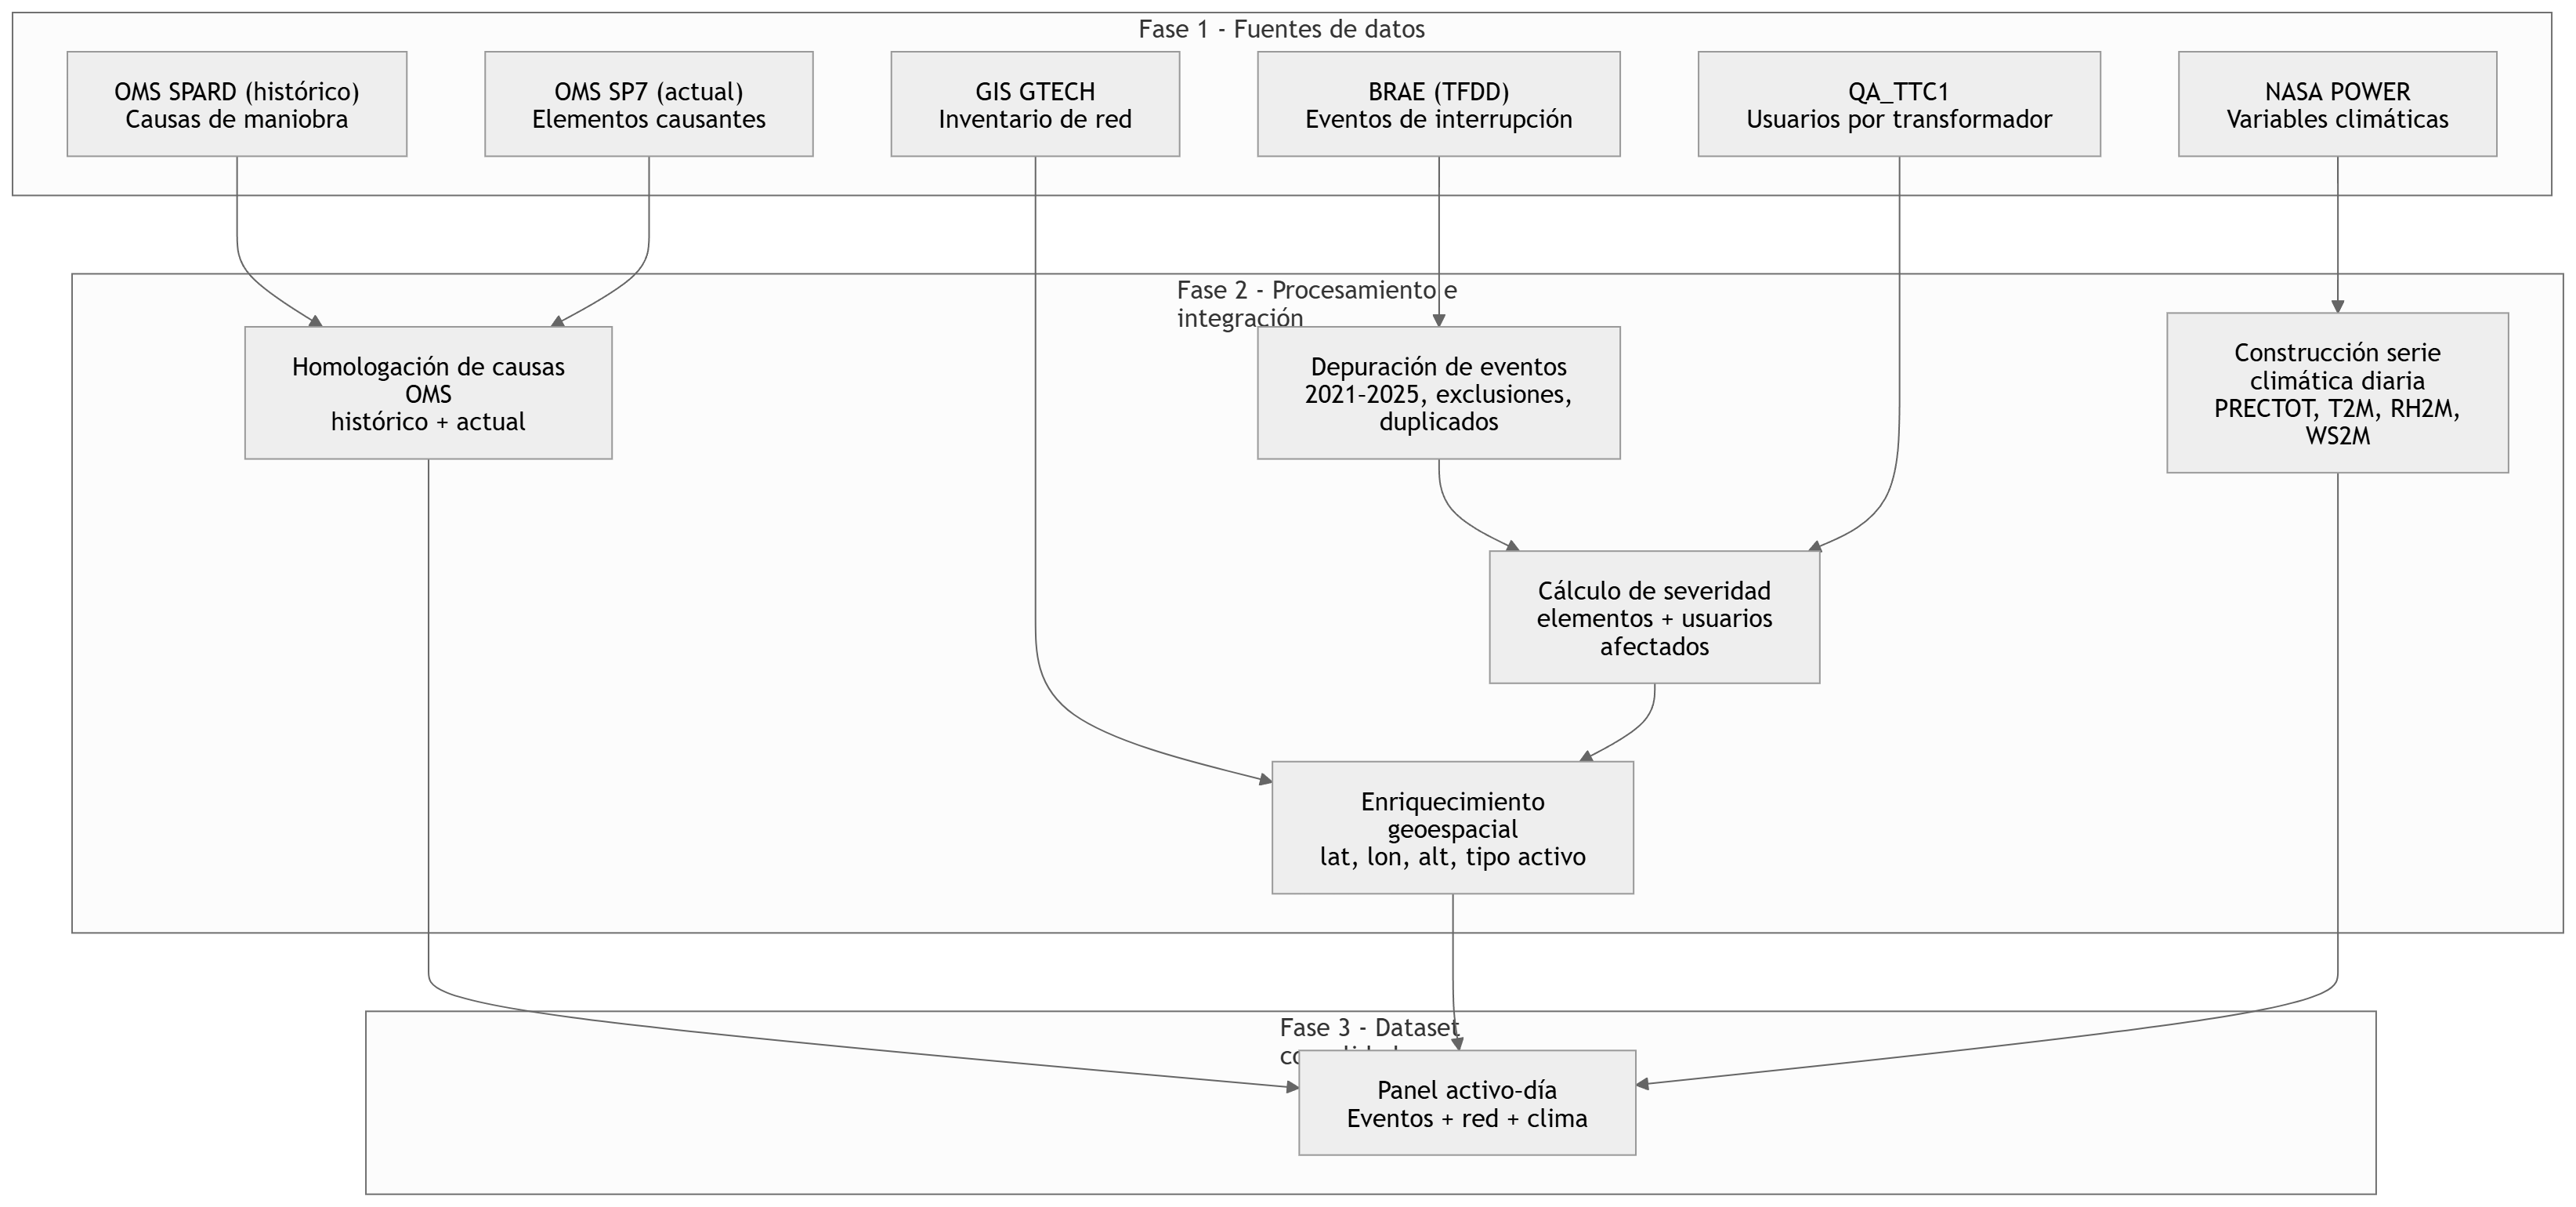
\includegraphics[width=\textwidth]{img/drawings/mermaid-diagram (1).png}
    \caption{Estructura del panel de datos activo–día}
    \label{fig:panel_activo_dia}
\end{figure}

\section{Código de extracción de datos}
\label{app:codigo}

Esta sección consolida el código de extracción utilizado en la Etapa~1 de la metodología (consultas SQL y fragmentos Python). En el cuerpo del documento se describe el procedimiento y se referencia el listado correspondiente.

\subsection{Consultas SQL}

\subsubsection{Eventos de interrupción (BRAE)}
\label{app:sql-brae}

\begin{lstlisting}[style=thesiscode,language=SQL,caption={Consulta SQL de extracción y depuración de eventos de interrupción (BRAE)},label={lst:sql_brae}]
SELECT DISTINCT FDD_CODIGOEVENTO AS ID_EVENTO
      ,FDD_FINICIAL AS FECHA_DESCONEXION
      ,FDD_FFINAL AS FECHA_CONEXION
      ,'' AS ELEMENTO_FALLADO
FROM BRAE.QA_TFDDREGISTRO
WHERE TO_CHAR(FDD_FINICIAL,'YYYY') IN ('2021', '2022', '2023', '2024', '2025')
  AND FDD_EXCLUSION = 'NO EXCLUIDA'
  AND FDD_CAUSA_SSPD NOT IN (1)
  AND FDD_FFINAL IS NOT NULL;
\end{lstlisting}

\subsubsection{Afectación por evento (BRAE + QA\_TTC1)}
\label{app:sql-afectacion}

\begin{lstlisting}[style=thesiscode,language=SQL,caption={Consulta SQL de afectación por evento (elementos y usuarios)},label={lst:sql_afectacion}]
SELECT FDD_CODIGOEVENTO AS ID_EVENTO
      ,COUNT(FDD_CODIGOELEMENTO) AS CANTIDAD_ELEMENTOS_FALLADOS
      ,SUM(CANTIDAD_USUARIOS) AS CANTIDAD_USUARIOS
FROM BRAE.QA_TFDDREGISTRO
LEFT JOIN (
    SELECT TC1_CODCONEX AS TRANSFORMADOR
          ,COUNT(TC1_CODCONEX) AS CANTIDAD_USUARIOS
          ,TC1_PERIODO AS PERIODO
    FROM QA_TTC1
    WHERE SUBSTR(TC1_PERIODO, 1, 4) IN ('2021', '2022', '2023', '2024', '2025')
    GROUP BY TC1_PERIODO, TC1_CODCONEX
) ON FDD_CODIGOELEMENTO = TRANSFORMADOR
 AND FDD_PERIODO_TC1 = PERIODO
WHERE TO_CHAR(FDD_FINICIAL,'YYYY') IN ('2021', '2022', '2023', '2024', '2025')
  AND FDD_EXCLUSION = 'NO EXCLUIDA'
  AND FDD_CAUSA_SSPD NOT IN (1)
  AND FDD_FFINAL IS NOT NULL
GROUP BY FDD_CODIGOEVENTO;
\end{lstlisting}

\subsubsection{Elemento causante histórico (OMS SPARD)}
\label{app:sql-oms-historico}

\begin{lstlisting}[style=thesiscode,language=SQL,caption={Consulta SQL del elemento causante histórico (OMS SPARD)},label={lst:sql_oms_historico}]
SELECT CODE AS CODIGO_MANIOBRA
      ,BREAKER AS ELEMENTO_FALLADO
FROM OMS.MANIOBRAS@SPARD
WHERE TO_NUMBER(TO_CHAR(FECHA, 'YYYY')) >= 2021
  AND CAUSA != 'PRUEBA';
\end{lstlisting}

\subsubsection{Inventario georreferenciado (GIS GTECH)}
\label{app:sql-gis}

\begin{lstlisting}[style=thesiscode,language=SQL,caption={Consulta SQL del inventario georreferenciado de activos (GIS GTECH)},label={lst:sql_gis}]
SELECT 
    nodo_transform_v AS ELEMENTO,
    coor_gps_lat     AS LATITUD,
    coor_gps_lon     AS LONGITUD,
    coor_z           AS ALTITUD,
    'Transformador'  AS TIPO,
    ubicacion
FROM ccomun@gtech c
JOIN cconectividad_e@gtech USING (g3e_fid)
WHERE c.estado = 'OPERACION'
  AND c.g3e_fno = 20400
UNION
SELECT 
    r.codigo         AS ELEMENTO,
    coor_gps_lat     AS LATITUD,
    coor_gps_lon     AS LONGITUD,
    coor_z           AS ALTITUD,
    'Reconectador'   AS TIPO,
    ubicacion
FROM ereconec_at@gtech r
JOIN ccomun@gtech c USING (g3e_fid)
JOIN cconectividad_e@gtech USING (g3e_fid)
WHERE c.estado = 'OPERACION';
\end{lstlisting}

\noindent La consulta del Listado~\ref{lst:sql_gis} se replica de forma análoga para Interruptor, Cuchilla, Aisladero, Reconectador y Transformador, homologando el tipo de activo en cada bloque \texttt{UNION}.

\subsection{Fragmentos Python}

\subsubsection{Elemento causante actual (OMS SP7)}
\label{app:py-oms-sp7}

\begin{lstlisting}[style=thesiscode,language=Python,caption={Fragmento Python de lectura y depuración del elemento causante actual (OMS SP7)},label={lst:py_oms_sp7}]
columnas_necesarias = ['Maniobra Apertura', 'Tipo Elemento', 'Elemento_Falla']
df = pd.read_csv(ruta_actual)
df.columns = df.columns.str.strip()
df = df[columnas_necesarias].drop_duplicates()
\end{lstlisting}

\subsubsection{Parámetros meteorológicos (NASA POWER)}
\label{app:py-nasa}

\begin{lstlisting}[style=thesiscode,language=Python,caption={Definición de parámetros meteorológicos extraídos de NASA POWER},label={lst:py_nasa}]
parametros_nasa = ("PRECTOT", "T2M", "T2M_MAX", "T2M_MIN", "RH2M", "WS2M")
\end{lstlisting}

\section{Informes reproducibles (HTML)}
\label{app:informes-html}

Los procedimientos de extracción, integración y análisis exploratorio descritos en la metodología se documentan de forma reproducible en informes HTML publicados en el repositorio del proyecto (GitHub Pages). En el cuerpo del documento se cita el apartado correspondiente de este apéndice; los hipervínculos a cada informe se concentran aquí.

\subsection{Consolidación del panel activo--día}
\label{app:html-consolidada}
Informe \texttt{Consolidada.html}: detalle de los pasos~\ref{paso:int-4} a~\ref{paso:int-8} de integración hacia el panel consolidado.
\href{\urlconsolidada}{Abrir informe}.

\subsection{Agrupación cuadrante $\times$ semana}
\label{app:html-agrupacion}
Informe \texttt{data\_agrupacion.html}: construcción de la tabla de análisis a grano cuadrante~$\times$~semana.
\href{\urlagrupacion}{Abrir informe}.

\subsection{Datos faltantes (tabla agrupada)}
\label{app:html-faltantes-agrupada}
Informe \texttt{missing\_values\_grouped.html}: diagnóstico de valores faltantes en \texttt{data\_agrupada.csv}.
\href{\urlfaltantesagrupada}{Abrir informe}.

\subsection{Valores extremos (panel consolidado)}
\label{app:html-outliers}
Informe \texttt{detection\_outliers.html}: identificación de valores extremos en el panel activo~$\times$~día.
\href{\urldetectionoutliers}{Abrir informe}.

\subsection{Valores extremos (tabla agrupada)}
\label{app:html-outliers-agrupada}
Informe \texttt{outliers\_gruped.html}: identificación de valores extremos en la tabla cuadrante~$\times$~semana.
\href{\urloutliersagrupada}{Abrir informe}.

\subsection{Estadísticos descriptivos}
\label{app:html-descriptivos}
Informe \texttt{calculo\_estadistico\_descriptivo.html}: cálculo de estadísticos descriptivos sobre la tabla agrupada.
\href{\urlestadisticosdescriptivos}{Abrir informe}.

\subsection{Distribución de variables}
\label{app:html-distribucion}
Informe \texttt{distribucion\_variables.html}: análisis de la forma de las distribuciones (densidades, asimetría, curtosis y ceros).
\href{\urldistribucionvariables}{Abrir informe}.

\subsection{Análisis temporal de eventos}
\label{app:html-temporal}
Informe \texttt{analisis\_temporal\_eventos.html}: series semanales, estacionalidad y autocorrelación de eventos.
\href{\urlanalisistemporal}{Abrir informe}.

\subsection{Emparejamiento evento--elemento}
\label{app:html-emparejamiento}
Informe \texttt{emparejamiento\_eventos.html}: cobertura anual de la trazabilidad entre eventos BRAE e inventario GIS.
\href{\urlemparejamientoeventos}{Abrir informe}.

\subsection{Materialización de $D_{\mathrm{mod}}$}
\label{app:html-datamod}
Informe \texttt{consolidado\_data\_mod.html}: filtro y exportación del dataset de modelado 2024--2025.
\href{\urlconsolidadodatamod}{Abrir informe}.

\subsection{Identificación de patrones}
\label{app:html-patrones}
Informe \texttt{identificacion\_patrones.html}: patrones temporales, espaciales y clima--evento sobre $D_{\mathrm{mod}}$.
\href{\urlidentificacionpatrones}{Abrir informe}.

\subsection{Análisis de correlación}
\label{app:html-correlacion}
Informe \texttt{analisis\_correlacion.html}: asociaciones de Spearman entre variables climáticas y operativas.
\href{\urlanalisisCorrelacion}{Abrir informe}.

\subsection{Análisis multivariado}
\label{app:html-multivariado}
Informe \texttt{analisis\_multivariado.html}: VIF, PCA, agrupamiento jerárquico y GLM Poisson exploratorio.
\href{\urlanalisisMultivariado}{Abrir informe}.

\subsection{Segmentación exploratoria}
\label{app:html-segmentacion}
Informe \texttt{segmentacion\_exploratoria.html}: perfiles por nivel de actividad, régimen de lluvia y clustering de cuadrantes.
\href{\urlsegmentacionexploratoria}{Abrir informe}.

\subsection{EDA consolidado}
\label{app:html-eda}
Informe \texttt{EDA.html}: síntesis ejecutiva del análisis exploratorio (Etapa~3) con hallazgos y lineamientos para la Etapa~4.
\href{\urlEDA}{Abrir informe}.

\subsection{Asociación y depuración de variables cuantitativas}
\label{app:html-asociacion-cuanti}
Informe \texttt{asociacion\_depuracion\_cuantitativas.html}: depuración \emph{ex ante} de covariables cuantitativas y exportación de la matriz de diseño.
\href{\urlasociaciondepuracioncuanti}{Abrir informe}.

\subsection{Justificación de la agregación espacial}
\label{app:html-etapa2-03}
Informe \texttt{Etapa2\_03\_justificacion\_agregacion\_espacial.html}: justificación del grano cuadrante~$\times$~semana y evidencia de concentración espacial de fallas.
\href{\urlEtapaDosTres}{Abrir informe}.

\subsection{Infraestructura eléctrica por cuadrante}
\label{app:html-etapa2-04}
Informe \texttt{Etapa2\_04\_infraestructura\_gis\_cuadrante.html}: agregación de tipologías y conteos de infraestructura GIS al polígono de cada cuadrante.
\href{\urlEtapaDosCuatro}{Abrir informe}.

\subsection{Estratificación municipal}
\label{app:html-etapa2-05}
Informe \texttt{Etapa2\_05\_estratificacion\_municipal.html}: asignación espacial de municipio y estrato predominante a cuadrantes reales.
\href{\urlEtapaDosCinco}{Abrir informe}.

\subsection{Eventos catastróficos UNGRD}
\label{app:html-etapa2-06}
Informe \texttt{Etapa2\_06\_desastres\_ungrd.html}: integración de emergencias UNGRD a municipio/cuadrante y semana.
\href{\urlEtapaDosSeis}{Abrir informe}.

\subsection{Sismicidad SGC}
\label{app:html-etapa2-07}
Informe \texttt{Etapa2\_07\_sismicidad\_sgc.html}: incorporación de sismicidad del SGC como exposición territorial del panel.
\href{\urlEtapaDosSiete}{Abrir informe}.

\subsection{Topología de red eléctrica}
\label{app:html-etapa2-08}
Informe \texttt{Etapa2\_08\_topologia\_red.html}: métricas topológicas de red por cuadrante y vecindad espacial/eléctrica.
\href{\urlEtapaDosOcho}{Abrir informe}.

\subsection{Integración del panel final}
\label{app:html-etapa2-09}
Informe \texttt{Etapa2\_09\_integracion\_panel\_final.html}: unión de fuentes enriquecidas hacia el panel base de modelado.
\href{\urlEtapaDosNueve}{Abrir informe}.

\subsection{Cargue NASA POWER semanal}
\label{app:html-etapa2-10}
Informe \texttt{Etapa2\_10\_cargue\_nasa\_semana.html}: cargue de variables climáticas NASA POWER agregadas por semana.
\href{\urlEtapaDosDiez}{Abrir informe}.

\subsection{Cargue de eventos semanales}
\label{app:html-etapa2-11}
Informe \texttt{Etapa2\_11\_cargue\_eventos\_semana.html}: agregación de eventos y métricas de continuidad a cuadrante--semana.
\href{\urlEtapaDosOnce}{Abrir informe}.

\subsection{Unión del panel semanal}
\label{app:html-etapa2-12}
Informe \texttt{Etapa2\_12\_union\_panel\_semana.html}: unión semanal de clima, eventos y atributos territoriales.
\href{\urlEtapaDosDoce}{Abrir informe}.

\subsection{Modelo espacial de SAIDI}
\label{app:html-etapa5-01}
Informe \texttt{Etapa5\_01\_modelo\_SAIDI\_espacial.html}: estimación, validación e interpretación del modelo espacial de SAIDI.
\href{\urlEtapaCincoUno}{Abrir informe}.

\subsection{Modelo espacial de SAIFI}
\label{app:html-etapa5-02}
Informe \texttt{Etapa5\_02\_modelo\_SAIFI\_espacial.html}: estimación, validación e interpretación del modelo espacial de SAIFI.
\href{\urlEtapaCincoDos}{Abrir informe}.

\section{Muestra completa de tablas base del proyecto}
\label{app:muestra-tablas-base}

Esta sección presenta, con todas las columnas y divididas en los bloques temáticos originales, las muestras ilustrativas de las dos tablas base descritas en la Etapa~2 de la metodología (Secciones~\ref{sec:logica_integracion} y~\ref{sec:agrupacion_cuadrante_semana}). Las vistas previas de estas mismas filas, con un subconjunto representativo de columnas, se presentan en el cuerpo del documento (Tablas~\ref{tab:muestra_consolidado_preview} y~\ref{tab:muestra_semanal_preview}).

\subsection{Tabla base consolidada (activo--día)}
\label{app:muestra-consolidado-completa}

\begin{table}[!htbp]
\centering
    \small
    \caption{Muestra de la tabla base consolidada (grano activo--día) -- Parte 1: activo y fecha}
    \label{tab:muestra_consolidado_final_1}
    \begin{tabular}{l l r r r l}
    \toprule
    \textbf{Id activo} & \textbf{Tipo} & \textbf{Lat.} & \textbf{Lon.} & \textbf{Alt.} & \textbf{Fecha día} \\
    \midrule
    AASW4819 & Aisladero      & 8.5786778 & -72.92349 & 219  & 01/01/2021 \\
    1T12452  & Transformador  & 8.5839989 & -72.92248 & 241  & 01/01/2021 \\
    REC21365 & Reconectador   & 8.5840628 & -72.92246 & 241  & 01/01/2021 \\
    CUC12345 & Cuchilla       & 7.7523729 & -73.23971 & 1236 & 01/01/2021 \\
    INT39845 & Interruptor    & 7.7476080 & -73.25551 & 1359 & 02/01/2021 \\
    AASW4820 & Aisladero      & 7.7561057 & -73.26037 & 1169 & 02/01/2021 \\
    1T12453  & Aisladero      & 7.7409332 & -73.20825 & 1636 & 02/01/2021 \\
    REC21366 & Transformador  & 7.7428641 & -73.18990 & 1542 & 02/01/2021 \\
    CUC12346 & Reconectador   & 7.7538839 & -73.17721 & 1707 & 03/01/2021 \\
    \bottomrule
    \end{tabular}
    \end{table}

\begin{table}[!htbp]
\centering
    \small
    \caption{Muestra de la tabla base consolidada (grano activo--día) -- Parte 2: severidad y clima inicial (continuación)}
    \label{tab:muestra_consolidado_final_2}
    \begin{tabular}{l l r r r r}
    \toprule
    \textbf{Id activo} & \textbf{Fecha día} & \textbf{C. elem.} & \textbf{C. usu.} & \textbf{Vel. viento} & \textbf{Temp. med.} \\
    \midrule
    AASW4819 & 01/01/2021 & 0   & 0    & 1.11 & 23.91 \\
    1T12452  & 01/01/2021 & 0   & 0    & 1.23 & 24.58 \\
    REC21365 & 01/01/2021 & 125 & 2015 & 0.96 & 23.04 \\
    CUC12345 & 01/01/2021 & 0   & 0    & 0.81 & 23.02 \\
    INT39845 & 02/01/2021 & 0   & 0    & 1.05 & 23.83 \\
    AASW4820 & 02/01/2021 & 0   & 0    & 1.12 & 24.08 \\
    1T12453  & 02/01/2021 & 0   & 0    & 1.08 & 24.52 \\
    REC21366 & 02/01/2021 & 0   & 0    & 1.26 & 24.37 \\
    CUC12346 & 03/01/2021 & 0   & 0    & 1.41 & 24.34 \\
    \bottomrule
    \end{tabular}
    \end{table}

\begin{table}[!htbp]
\centering
    \small
    \caption{Muestra de la tabla base consolidada (grano activo--día) -- Parte 3: clima complementario (continuación)}
    \label{tab:muestra_consolidado_final_3}
    \begin{tabular}{l l r r r r}
    \toprule
    \textbf{Id activo} & \textbf{Fecha día} & \textbf{Hum. rel.} & \textbf{Temp. min.} & \textbf{Temp. max.} & \textbf{Precip.} \\
    \midrule
    AASW4819 & 01/01/2021 & 78.91 & 20.06 & 29.98 & 3.19 \\
    1T12452  & 01/01/2021 & 75.79 & 20.27 & 30.90 & 1.31 \\
    REC21365 & 01/01/2021 & 83.94 & 20.26 & 27.82 & 3.19 \\
    CUC12345 & 01/01/2021 & 79.55 & 17.92 & 30.09 & 7.28 \\
    INT39845 & 02/01/2021 & 69.70 & 19.35 & 30.79 & 1.99 \\
    AASW4820 & 02/01/2021 & 61.99 & 17.20 & 30.81 & 0.98 \\
    1T12453  & 02/01/2021 & 72.16 & 20.38 & 30.59 & 2.70 \\
    REC21366 & 02/01/2021 & 75.50 & 20.18 & 30.63 & 3.29 \\
    CUC12346 & 03/01/2021 & 74.34 & 20.40 & 30.43 & 1.86 \\
    \bottomrule
    \end{tabular}
    \end{table}

\begin{table}[!htbp]
\centering
    \small
    \caption{Muestra de la tabla base consolidada (grano activo--día) -- Parte 4: variables de continuidad (continuación)}
    \label{tab:muestra_consolidado_final_4}
    \begin{tabular}{r r}
    \toprule
    \textbf{Duración (min)} & \textbf{Frecuencia} \\
    \midrule
    0     & 0 \\
    0     & 0 \\
    421.5 & 3 \\
    0     & 0 \\
    0     & 0 \\
    0     & 0 \\
    0     & 0 \\
    0     & 0 \\
    0     & 0 \\
    \bottomrule
    \end{tabular}
    \end{table}

\noindent\textit{Nota:} las filas de las Tablas~\ref{tab:muestra_consolidado_final_1} a~\ref{tab:muestra_consolidado_final_4} corresponden al mismo conjunto de observaciones en el mismo orden.

\subsection{Tabla base semanal cuadrante}
\label{app:muestra-semanal-completa}

\begin{table}[!htbp]
\centering
    \small
    \caption{Muestra de la tabla base semanal cuadrante (grano cuadrante--semana) -- Parte 1: cuadrante, semana, coordenadas e impacto operativo}
    \label{tab:muestra_semanal_cuadrante_1}
    \begin{tabular}{r l r r r r r}
    \toprule
    \textbf{Id cuad.} & \textbf{Semana} & \textbf{Lat.} & \textbf{Lon.} & \textbf{Alt.} & \textbf{Usu. afect.} & \textbf{Elem. afect.} \\
    \midrule
      1 & 28/12/2020 & 7.0012 & -72.6855 & 3418 &    0 &   0 \\
      1 & 04/01/2021 & 7.0012 & -72.6855 & 3418 &    0 &   0 \\
      3 & 04/01/2021 & 7.1548 & -72.7196 & 2850 &    0 &   0 \\
     12 & 11/01/2021 & 7.4521 & -72.8903 & 1240 &  842 &  18 \\
     45 & 18/01/2021 & 7.7539 & -73.1204 &  890 &    0 &   0 \\
    117 & 25/01/2021 & 7.9215 & -72.5021 &  286 & 1254 &  24 \\
    203 & 01/02/2021 & 8.0812 & -72.4108 &  312 &    0 &   0 \\
     45 & 08/02/2021 & 7.7539 & -73.1204 &  890 &  315 &   6 \\
    117 & 15/02/2021 & 7.9215 & -72.5021 &  286 &  680 &  11 \\
    \bottomrule
    \end{tabular}
    \end{table}

\begin{table}[!htbp]
\centering
    \small
    \caption{Muestra de la tabla base semanal cuadrante (grano cuadrante--semana) -- Parte 2: temperatura (continuación)}
    \label{tab:muestra_semanal_cuadrante_2}
    \begin{tabular}{r l r r r}
    \toprule
    \textbf{Id cuad.} & \textbf{Semana} & \textbf{Temp. med.} & \textbf{Temp. max.} & \textbf{Temp. min.} \\
    \midrule
      1 & 28/12/2020 & 13.6 & 19.8 &  6.2 \\
      1 & 04/01/2021 & 12.8 & 18.5 &  5.8 \\
      3 & 04/01/2021 & 13.1 & 19.2 &  6.0 \\
     12 & 11/01/2021 & 22.4 & 28.6 & 16.8 \\
     45 & 18/01/2021 & 23.8 & 30.1 & 18.2 \\
    117 & 25/01/2021 & 24.1 & 30.4 & 18.9 \\
    203 & 01/02/2021 & 24.5 & 30.8 & 19.1 \\
     45 & 08/02/2021 & 23.5 & 29.7 & 17.8 \\
    117 & 15/02/2021 & 24.3 & 30.2 & 18.6 \\
    \bottomrule
    \end{tabular}
    \end{table}

\begin{table}[!htbp]
\centering
    \small
    \caption{Muestra de la tabla base semanal cuadrante (grano cuadrante--semana) -- Parte 3: clima complementario (continuación)}
    \label{tab:muestra_semanal_cuadrante_3}
    \begin{tabular}{r l r r r r}
    \toprule
    \textbf{Id cuad.} & \textbf{Semana} & \textbf{Hum. med.} & \textbf{Vel. med.} & \textbf{Vel. max.} & \textbf{Precip.} \\
    \midrule
      1 & 28/12/2020 & 82.4 & 1.15 & 2.31 & 18.5 \\
      1 & 04/01/2021 & 80.1 & 1.08 & 2.18 & 12.3 \\
      3 & 04/01/2021 & 81.6 & 1.12 & 2.25 & 15.7 \\
     12 & 11/01/2021 & 76.3 & 0.98 & 1.95 &  8.4 \\
     45 & 18/01/2021 & 74.8 & 1.05 & 2.10 &  6.2 \\
    117 & 25/01/2021 & 73.5 & 1.18 & 2.42 &  9.8 \\
    203 & 01/02/2021 & 72.9 & 1.22 & 2.55 &  4.1 \\
     45 & 08/02/2021 & 75.2 & 1.09 & 2.08 & 11.6 \\
    117 & 15/02/2021 & 74.1 & 1.14 & 2.35 &  7.3 \\
    \bottomrule
    \end{tabular}
    \end{table}

\begin{table}[!htbp]
\centering
    \small
    \caption{Muestra de la tabla base semanal cuadrante (grano cuadrante--semana) -- Parte 4: continuidad del servicio (continuación)}
    \label{tab:muestra_semanal_cuadrante_4}
    \begin{tabular}{r r}
    \toprule
    \textbf{N eventos} & \textbf{Duración total (h)} \\
    \midrule
     0 &   0.0 \\
     0 &   0.0 \\
     0 &   0.0 \\
     5 &  28.4 \\
     0 &   0.0 \\
     8 &  41.7 \\
     0 &   0.0 \\
     2 &  12.6 \\
     4 &  22.3 \\
    \bottomrule
    \end{tabular}
    \end{table}

\noindent\textit{Nota:} las filas de las Tablas~\ref{tab:muestra_semanal_cuadrante_1} a~\ref{tab:muestra_semanal_cuadrante_4} corresponden al mismo conjunto de observaciones en el mismo orden. Cadena de unidades de continuidad: panel diario en minutos (\texttt{DURACION\_min}) $\rightarrow$ conversión \texttt{/60} $\rightarrow$ \texttt{duracion\_total} semanal en horas.
